\documentclass[a4paper,pdftex]{paper}
\usepackage{verbatim}
\usepackage{graphicx}
\usepackage{color}
\usepackage{courier}
\usepackage{booktabs}
\usepackage{varioref}
%\usepackage{savetrees}
\usepackage{float}
\floatplacement{figure}{ht}
\floatplacement{table}{ht} 
\floatstyle{ruled}
%\restylefloat{table}
\usepackage{listings}
\usepackage{hyperref}

\definecolor{comment}{rgb}{.23922,.38039,.16078}
\definecolor{keyword}{rgb}{.098039,.098039,.439216}
\definecolor{string}{rgb}{0,.4,0}


\def\regaccess{{\tt regaccess}}
\setlength{\parindent}{0pt}
\setlength{\parskip}{10pt plus 6pt minus 4pt}


\lstset{language=XML,
  morekeywords={schema,element,key,keyref,selector,field},
  basicstyle=\small\tt,
  keywordstyle=\textbf,
  breaklines=true,
  breakatwhitespace=true,
  breakautoindent=true,
  tabsize=4,
  keywordstyle=\color{keyword}\textbf,
  commentstyle=\color{comment}\textit,
  stringstyle=\color{string},
  rulesepcolor=\color{black}}


\lstdefinelanguage{CSharp}
{
 morecomment = [l]{//}, 
 morecomment = [l]{///},
 morecomment = [s]{/*}{*/},
 morestring=[b]", 
 sensitive = true,
 morekeywords = {abstract,  event,  new,  struct,
   as,  explicit,  null,  switch,
   base,  extern,  object,  this,
   bool,  false,  operator,  throw,
   break,  finally,  out,  true,
   byte,  fixed,  override,  try,
   case,  float,  params,  typeof,
   catch,  for,  private,  uint,
   char,  foreach,  protected,  ulong,
   checked,  goto,  public,  unchecked,
   class,  if,  readonly,  unsafe,
   const,  implicit,  ref,  ushort,
   continue,  in,  return,  using,
   decimal,  int,  sbyte,  virtual,
   default,  interface,  sealed,  volatile,
   delegate,  internal,  short,  void,
   do,  is,  sizeof,  while,
   double,  lock,  stackalloc,   
   else,  long,  static,   
   enum,  namespace,  string}
}

\hypersetup{
  pdftitle={regaccess},
  pdfauthor={mru},
  pdfkeywords={avr, microcontroller, serial communication},
%  bookmarksnumbered,
%  bookmarks=true,
  colorlinks=false,
  breaklinks=true,
  pdfborder=0 0 0,
%  bookmarksopen=false,
}


\title{regaccess - Simple PC to uC communication}
\author{mru}
\date{\today{}}

\begin{document}
\thispagestyle{empty}
\maketitle{}

\begin{abstract}
  \regaccess{} provides a simple mechanism for remote method
  invocation from a PC to a microcontroller by generating code for the
  controller and the host application (currently for python and c\#).
  Besides the function calling capabilities it also provides a
  multi-type register based programming model, allowing easy
  communication with automatic persistance of register values.
\end{abstract}

\tableofcontents{}
\section{Introduction}
\label{sec:intro}


\regaccess{} implements two ways to establish communication between a
PC (master) and a micro controller (slave).  Firstly, a register
abstraction and secondly a function invocation abstraction is
provided.  Communication is done over a serial (RS232) line.

Available registers and callable functions are defined in an simple
XML format and code for both sides (slaver and master) is generated.

\begin{figure}
  \centering
  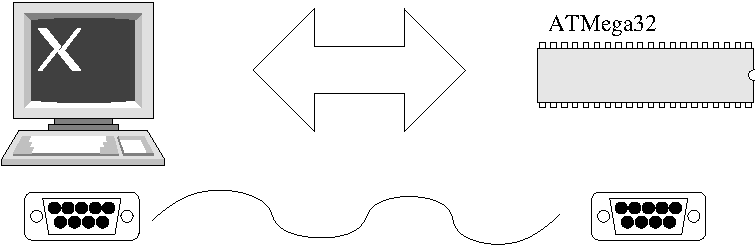
\includegraphics[width=0.5\textwidth]{communication.pdf}
  \caption{Schematic}
  \label{fig:schem}
\end{figure}

\section{Architectural Overview}

\begin{figure}
  \centering
  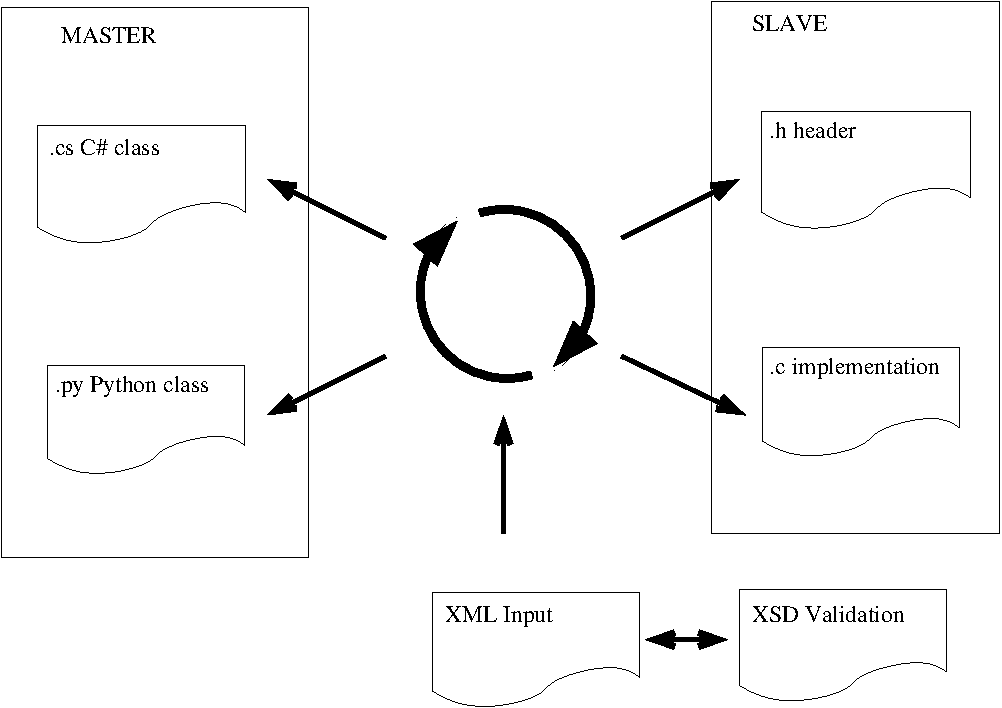
\includegraphics[width=0.7\textwidth]{gen_overview.pdf}
  \caption{Architecture}
  \label{fig:arch}
\end{figure}

The program is implemented in Python 2.5.  Mako
templates\footnote{\url{www.makotemplates.org/}} are used to generate
the output.  Table \vref{tab:versions} shows the used software
component versions.

\begin{table}
  \centering
  \begin{tabular}{ll} \toprule
    Component & Version \\ \midrule
    {\tt avr-gcc } & 4.3.4 \\
    {\tt python } & 2.6.5 \\
    {\tt mako } & 0.2.5 \\ \bottomrule
  \end{tabular}
  \caption{Version overview}
  \label{tab:versions}
\end{table}

\section{Register Model}

Several \emph{Register Files} can be defined.  Each File defines the
type of the contained registers.  Access modifiers can be defined for
individual registers.  Table \vref{tab:regprop} shows the supported
properties, the details are described in Section \vref{sec:inspec}.


\begin{table}
  \centering
  \begin{tabular}{lll} \toprule
    Property & Semantic  \\ \midrule
    {\tt type} & register type  \\
    {\tt init} & initial value for registers  \\
  \end{tabular}
  \caption{Register File Properties}
  \label{tab:regfileprop}
\end{table}


\begin{table}
  \centering
  \label{tab:regprop}
  \begin{tabular}{lll} \toprule
    Property & Semantic & Default Value \\ \midrule
    {\tt read} & allow read access & 1 \\
    {\tt write} & allow write access & 1 \\
    {\tt persist} & automatic EEPROM persitence & 0 \\
    {\tt default} & assign default value & n/a \\ \bottomrule
  \end{tabular}
  \caption{Register Properties}
\end{table}

\subsection{EEPROM Persistence}



\section{Function Invokation}

\section{Input Specification}
\label{sec:inspec}

The XML input is specified with a XML Schema Defintion file.
See \vref{sec:app_input_xsd}.

\section{Code Generation}

Mako is used to generate the output code.
See \vref{sec:mako_gen_avr_impl}.

\section{Serial Communication Protocol}

A Master-Slave communication protocol is implemented.  All
communication is initiated by the master (the PC).  The slave
(microcontroller) listens to the serial port and reacts to the
requests by the master.

Datagrams are sent byte-wise and for efficiency no strings are used.

A datagram sent by the master is sent as follows:

\begin{itemize}
\item An opcode is sent. This is one byte long
\item in-parameters of the functions are transmitted.
\item The slave responses with a status code
\item IF the status code is { \tt STATUS\_OK } AND the called function
  has out-parameters
  \begin{itemize}
  \item the out-parameters are transmitted from the slave to the host
  \end{itemize}
\end{itemize}

\subsection{Marshalling}

Supported Types:

\begin{itemize}
\item float
\item byte
\item short
\item ushort
\end{itemize}

\subsection{Status Codes}

\appendix{}
\section{Input Example}

\lstinputlisting[caption={Input Example}]{heater-control-regs.xml}

\section{Input Validation}
\label{sec:app_input_xsd}

\lstinputlisting[caption={The schema definition for the XML files}]{regaccess.xsd}

\section{A Mako Template}
\label{sec:mako_gen_avr_impl}


\lstinputlisting[language=C,caption={Template to generate the
  slave implementation}]{gen_avr_impl.mako}


\section{Generated Code examples: Slave header}
\label{sec:gen_out}

\lstinputlisting[language=C,caption={Slave header}]{regaccess.h}

\section{Generated Code examples: Slave implementation}

\lstinputlisting[language=C,caption={Slave implementation}]{regaccess.c}


\section{Generated Code examples: Master / CSharp}
\label{sec:gen_out_cs}

\lstinputlisting[language=CSharp,caption={Master CSharp}]{heatercontrol.cs}

\section{Generated Code examples: Master / Python}
\label{sec:gen_out_py}

\lstinputlisting[language=Python,caption={Master Python}]{heatercontrol.py}



\end{document}
